\documentclass[11pt]{article}
\usepackage[margin=1in]{geometry}
\usepackage[T1]{fontenc}
\usepackage{lmodern}
\usepackage{microtype}
\usepackage{amsmath}
\usepackage{booktabs}
\usepackage{tabularx}
\usepackage{graphicx}
\usepackage{caption}
\usepackage{enumitem}
\usepackage[numbers,sort&compress]{natbib}
\usepackage{xcolor}
\usepackage{placeins}
\usepackage{xurl}
\usepackage[colorlinks=true,linkcolor=blue!50!black,citecolor=blue!50!black,urlcolor=blue!50!black]{hyperref}
\setlist{itemsep=2pt,topsep=4pt}
\captionsetup{font=small,labelfont=bf}
\newcommand{\forum}[1]{\href{https://www.kaggle.com/competitions/gemma-4-developer-agent/discussion/#1}{forum #1}}

\title{\textbf{Runtime-Bound: What Limits a Local 31B Coding Agent, and What Local Evaluation Gets Wrong}\\[8pt]
\large On a fixed 12-hour, 32k-context scorer, the runtime decides more than the prompt, the adapter or the weights}
\author{shashanka\\\small Gemma 4 Developer Agent Paper Track\\\small Code: \url{https://github.com/shashanka300/runtime-bound}}
\date{November 2026}

\begin{document}
\maketitle

\begin{abstract}
We spent seven weeks and one consumer GPU (RTX 5090, 32\,GB) trying to improve a Gemma~4 31B (int4) software-engineering agent for a scorer that runs about 120 hidden tasks in 12 hours on 4$\times$L4 GPUs with a 32k context. We report what limited it. First, accounting: 90\% of the starter agent's failures were context exhaustion caused by one setting, a 16k output reserve inside a 32k window; fixing that line raised the local solve rate from 18.8\% to 31.3\% (paired, $p = 0.006$). Second, a fidelity ladder that moves local runs toward the scorer one condition at a time. It found three scorer-side defects (thinking budget never sent, earlier reasoning dropped from the prompt, LoRA weights wiped), all later confirmed or fixed by the organizers, and three local artefacts that would have misled us. Third, an anatomy of wall-clock: timed-out tasks lose 62\% of their time in 1--3 turns that think to the 4,096-token cap, half of them repetition loops. Fourth, ten agent-side interventions, from planning layers and sub-agents to self-generated LoRA and activation-guided weight edits, none of which beat the tuned single agent. The common cause is the runtime: the time cap, the context window and the way history is compacted. We release the tooling that made these measurements reproducible.
\end{abstract}

\section{Introduction}
Small open models are now good enough to fix real GitHub issues some of the time, and the Gemma~4 Developer Agent competition asks how far a 31B model can go under a fixed budget~\citep{gemma4paper2026}. The natural levers are the ones the submission format exposes: the system prompt, the agent graph, sampling, and LoRA adapters. Our thesis is that on this scorer these levers matter less than the runtime around the model: the wall-clock cap, the 32k window, how much of it is reserved for output, and how history is kept or compacted between turns.

We test the thesis with paired experiments on public tasks, reproduced on the scorer's own engine and harness. Contributions:
\begin{enumerate}
\item \textbf{Accounting (C1).} A token and failure taxonomy of 387 starter runs. One configuration line explains most failures, and fixing it gives the largest gain we measured.
\item \textbf{Fidelity ladder (C2).} A cumulative local-to-scorer decomposition that separates real scorer effects from local artefacts, with three defects reported to and fixed by the organizers.
\item \textbf{Wall-clock anatomy (C3).} Where the time goes in tasks that run out of it, and why simple caps do not recover it.
\item \textbf{Negative results (C4).} Ten interventions, each tested paired against the same baseline, including self-bootstrapped fine-tuning on a rented H100 and activation-guided weight edits.
\item \textbf{Measurement lessons (C5).} Why a public-task screen ranked our variants differently from the leaderboard, and what a reliable local proxy needs.
\end{enumerate}

\section{Setting}
\paragraph{Scorer.} The model is \texttt{gemma-4-31b-it-qat-w4a16-ct} served by vLLM~0.19.1~\citep{kwon2023vllm} on 4$\times$L4 with a 32,768-token window. Agents are declarative (YAML, prompts, sampling, tools from a closed registry, optional adapters) and run in Google ADK; each task gets an offline Docker sandbox, a tool-call cap and a per-task time cap, and the whole run must finish in 12 hours. A run that overruns it is reported to return no score (\forum{755677}). Hidden tasks come from repositories that are not in the public set (\forum{742882}).

\paragraph{Local replica.} One RTX 5090 serves the same checkpoint with the scorer's vLLM build and flags, installed from the organizers' wheelhouse, and the official harness (swegemma) runs the tasks. The L4 box decodes about 1.6$\times$ slower, so we scale the per-task cap by 0.625 (7\,min becomes 4.375\,min) and run one task at a time, as the scorer does.

\paragraph{Tasks.} 129 public tasks (fastapi 67, rich 48, requests 13, httpx 1). Only 41 can be graded offline with the released environment (Section~\ref{sec:measure}), so later screens use the 39 gradable, non-pathological tasks. For training data we also ingested 142 SWE-rebench tasks from other repositories.

\paragraph{Statistics.} Every comparison is paired on the same tasks: differences with bootstrap 95\% intervals and exact McNemar tests~\citep{agarwal2021rliable}. With 39--80 pairs, differences of $\pm$3 tasks are within noise, and we say so where it applies.

\section{Method: the fidelity ladder}
A local score is only useful if it predicts the scorer. Our first submission solved 31\% of tasks locally and scored 0.03 on the board. Instead of changing the agent, we moved the local setup toward the scorer one condition at a time, keeping the agent fixed and pairing each step with the previous one (Figure~\ref{fig:ladder}):
\begin{enumerate}
\item \textbf{Adapters.} A canary LoRA (random \texttt{lora\_B}) produced output identical to the base model on the scorer's original vLLM build: adapters were silently wiped. Removing the starter adapter locally changed nothing (30.0\% vs 30.0\%).
\item \textbf{Thinking translation.} The harness validated \texttt{thinking\_budget} but never sent it to vLLM; on the scorer, thinking was bounded only by \texttt{max\_output\_tokens}. Locally the effect was zero.
\item \textbf{Engine.} Replaying 164 recorded requests on both engines showed that vLLM~0.19.1 dropped the assistant's earlier \texttt{reasoning\_content} from the prompt (median 418 tokens shorter at turns 2--4, 2,583 from turn 5), so the model re-derived its plan every turn. The newer engine kept it and instead ran out of context. Stall-free, the two engines solved 27.5\% and 25.0\% (paired $-2.5$ [$-15$, $+10$]) and failed in opposite ways: 22 timeouts versus 35\% context deaths.
\end{enumerate}

\begin{figure}[t]
\centering
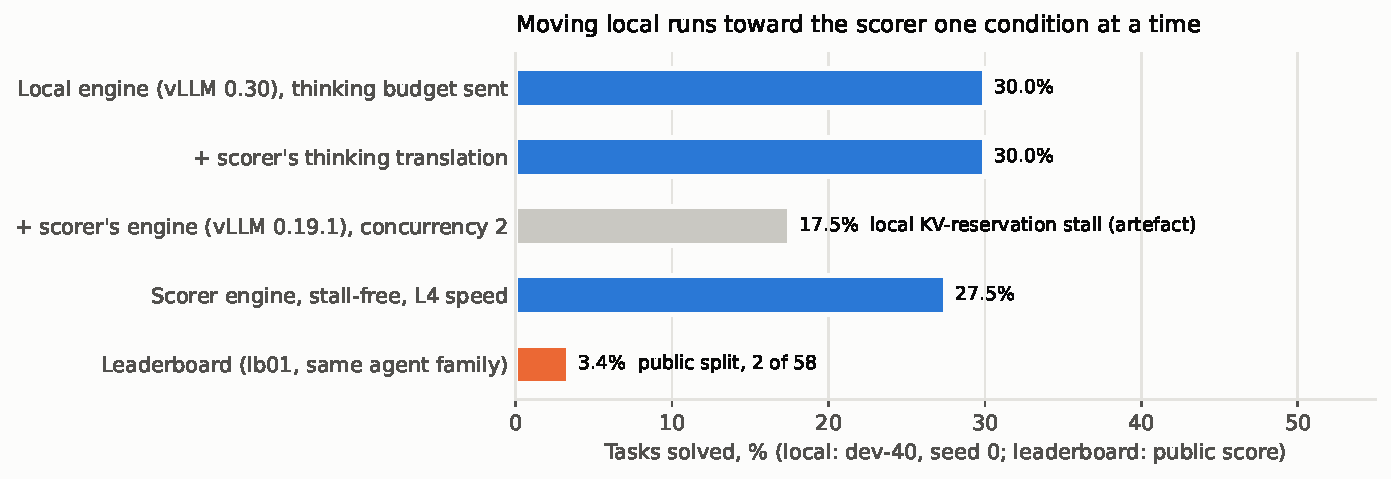
\includegraphics[width=\linewidth]{figures/fig1_fidelity_ladder.pdf}
\caption{The fidelity ladder. Each bar adds one scorer condition to the previous one (same agent, dev-40, seed 0). The grey bar is a local artefact, not a scorer effect. Even the stall-free scorer replica solves 8$\times$ more than the board.}
\label{fig:ladder}
\end{figure}

All three defects were reported on the competition forum and later confirmed or fixed (adapters load and thoughts are kept in the current wheelhouse). Three local artefacts nearly misled us and are worth naming because they are easy to repeat:
\begin{itemize}
\item \textbf{KV reservation.} vLLM's YAML config loader silently drops boolean \texttt{false}, so \texttt{scheduler-\allowbreak reserve-\allowbreak full-isl: false} was never applied. At concurrency 2 this produced request stalls that we first mistook for a 12.5-point engine effect.
\item \textbf{Wheel cache.} The harness caches unpacked dependency wheels under a fixed name that ignores which wheel set built it. It poisoned our first gradability sweep, and two months later a cache built from 1,450 SWE-rebench wheels broke pytest on every public task of an adapter screen (0/19 solved; the rerun with an isolated cache solved 9/32).
\item \textbf{Telemetry.} We log every run with a manifest and 1\,Hz GPU telemetry, so these artefacts were found by inspecting traces rather than by a lucky reading of a score.
\end{itemize}

\section{Results}
\subsection{Accounting: one line explained most failures (C1)}
Across 387 starter runs (129 tasks $\times$ 3 seeds, 6-minute cap) the agent solved 24.3\% [20.3, 28.8]. Of 250 failures, 90.4\% were context exhaustion; wrong edits were 6\% and mislocalization under 2\%. Token accounting located the cause: the starter sets \texttt{max\_output\_tokens: 16384}, which vLLM reserves out of the 32k window, leaving a 16k prompt that a few file reads fill. Truncated tool output was 21\% of prompt tokens and re-prefill after resets 13\%; re-reading files was only 2\%. One configuration line was worth more than any prompt or architecture change we tried later (Table~\ref{tab:e1b}).

\begin{table}[!htb]
\centering\footnotesize
\begin{tabular}{lccl}
\toprule
Arm (dev-40, 2 seeds) & Solved & Context deaths & Paired difference \\
\midrule
A starter & 18.8\% & 73.8\% & --- \\
B output reserve = thinking + 4,096 & \textbf{31.3\%} & 23.8\% & B$-$A \textbf{+12.5 [+5.0, +21.3]}, $p = 0.006$ \\
C = B + prompt guidance & 31.3\% & 25.0\% & C$-$B 0.0 \\
D = B + fresh-context retry & 32.5\% & 10.0\% & D$-$B +1.3, n.s. \\
\bottomrule
\end{tabular}
\caption{Context fixes (E1b). One setting, the output reserve, accounts for the gain.}
\label{tab:e1b}
\end{table}

\subsection{Context architecture: a phase agent does not help under the real budget (C4)}
Our pre-registered headline was a phase-decomposed agent (localize, reproduce, edit, verify) with fresh contexts per phase, designed so the window behaves like a prefix-closed cache~\citep{belady1966}. Under generous local budgets it tied the fixed single agent (+2.5 [$-3.8$, +10.0], 80 pairs; pre-registered bar +5). Its read-only localizer looped on identical tool calls in 28/79 runs (one grep 335 times) against 1/80 for the single agent, a near-greedy sampling effect (temperature 0.2) that Gemma's recommended sampling removed. Under scorer conditions the phase agent lost: 25.0\% and 17.5\% for two variants against 32.5\% for the single agent with thinking off ($-15$ [$-27.5$, $-2.5$] for the second). Splitting an already short budget across phases leaves each phase too little.

\subsection{Where the wall-clock goes (C3)}
On the fixed scorer engine our best configuration, lb04 (public recipe: thinking budget 4,096, temperature 0.2, 28 calls, 7\,min), solved 16/39 locally. Its 12 timed-out tasks look different from its solved ones (Table~\ref{tab:anatomy}, Figure~\ref{fig:anatomy}).

\begin{table}[!htb]
\centering\footnotesize
\begin{tabular}{lcccc}
\toprule
lb04, 39 tasks & Longest turn (median) & Turns $>$1,500 tokens & Time in 3 slowest turns & First edit (median) \\
\midrule
Solved (16) & 968 tokens & 0.3 & 42\% & 44\,s \\
Timed out (12) & 4,130 tokens (cap) & 1.8 & 62\% & 195\,s; 5 never edit \\
\bottomrule
\end{tabular}
\caption{Timed-out and solved tasks differ in a few very long turns, not in the number of turns.}
\label{tab:anatomy}
\end{table}

\begin{figure}[!htb]
\centering
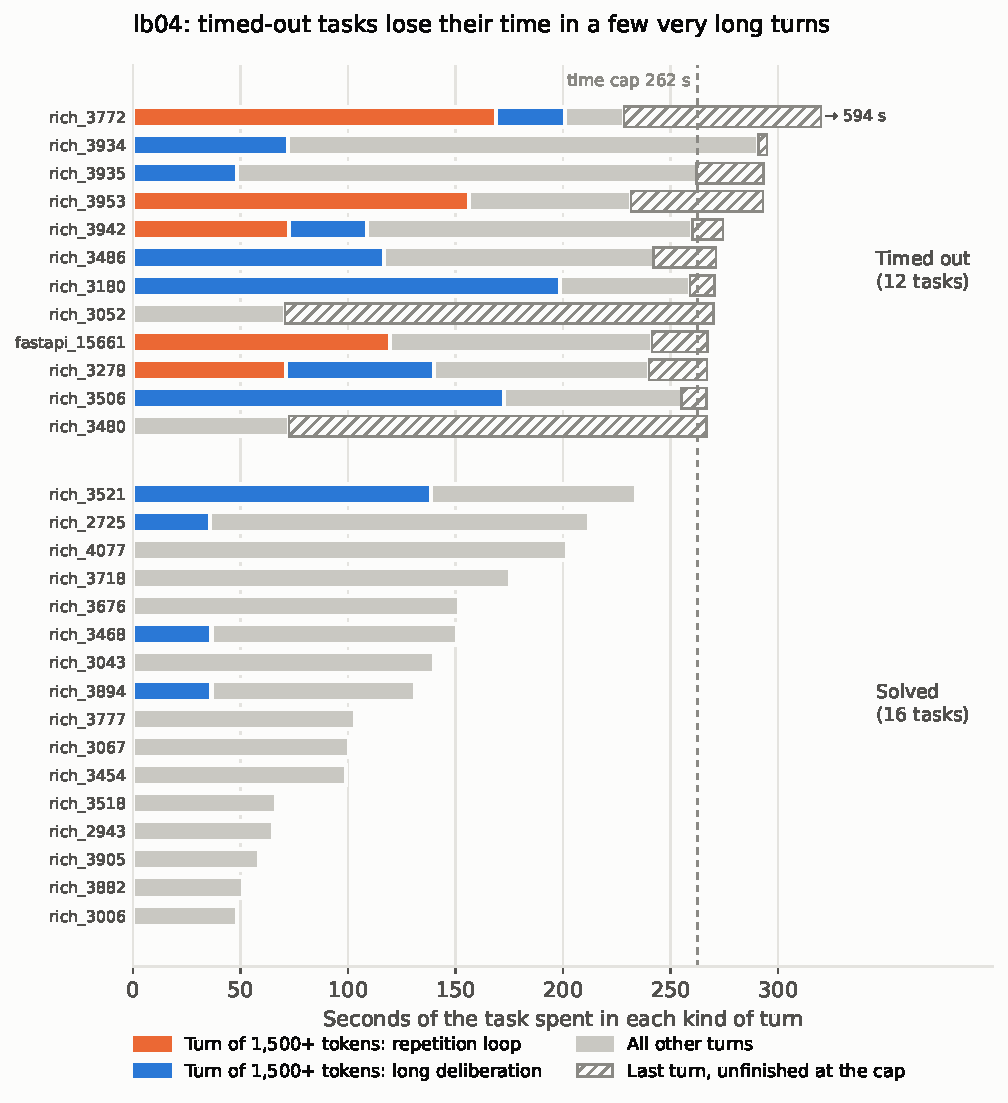
\includegraphics[width=0.7\linewidth]{figures/fig2_timeout_anatomy.pdf}
\caption{Where each task's time goes (lb04, the 12 timed-out and 16 solved tasks). Turns of 1,500+ output tokens are split into repetition loops (more than 25\% duplicated sentences) and long deliberation; the hatched segment is the final model call, still generating when the cap hit and therefore absent from the trace.}
\label{fig:anatomy}
\end{figure}

Of the 18 turns that reached 3,000 tokens, 8 were repetition loops (one repeated the same two sentences for 4,100 tokens), the rest long genuine deliberation. Two cheap fixes each address half the problem and lose elsewhere. Capping thinking at 2,048 removed the long turns but solved 12/39, since deliberation is sometimes what solves the task. Raising the temperature to 1.0 on the same 12 tasks cut loops from 7 to 1 and timeouts from 12 to 5, but most tasks then hit the call cap with wrong patches: 2 of the 12 were solved, against 0. We ran this arm only on the timed-out tasks, so what it costs on the tasks lb04 solves is unmeasured (Section~\ref{sec:limits}). On hard tasks the loop is a symptom of not knowing the fix, not the reason the fix is missing; this is the low-temperature degeneration described by \citet{holtzman2020degeneration}.

\subsection{Ten interventions that did not beat the tuned single agent (C4)}
All rows in Table~\ref{tab:interventions} are paired against lb04 on the same 39 tasks at scorer fidelity unless noted.

\begin{table}[h]
\centering\small
\begin{tabularx}{\linewidth}{Xcl}
\toprule
Intervention & Solved & Note \\
\midrule
lb04 baseline & 16/39 & board 0.15 \\
Thinking budget 2,048 & 12/39 & long turns gone, solves lost \\
Audit rules in the prompt & 14/39 & --- \\
No graph tools, 36 calls, 6 min, $T{=}1$ & 14/39 & time-capped 15 $\to$ 23 \\
Notes file in /tmp & 14/39 & slower (5.9 vs 5.5 scorer-min/task) \\
Skill helper scripts & 13/39 & empty patches 11 $\to$ 17 \\
Zero-call plan + status line & 15/39 & empty patches 11 $\to$ 9; \textbf{board 0.10} \\
Plan + forced edit by call 10 & 13/39 & empty patches 16 \\
Locator sub-agent & 12/39 & sub-agent used 13.9 of the shared 28 calls \\
Self-generated LoRA (r16, all linear layers) & 9/32 vs 12/32 & screen stopped at 32 tasks \\
Activation-guided weight edit (12B) & null & no edit cleared the bar without damage \\
12B with the same agent & 7/39 & --- \\
\bottomrule
\end{tabularx}
\caption{Interventions against the tuned single agent. Differences of $\pm$3 tasks are within noise.}
\label{tab:interventions}
\end{table}

\paragraph{Self-generated fine-tuning.} We rejection-sampled 113 solved runs (118 tasks, 5.3M tokens, the 39 screen tasks held out) from plain and hinted runs on public and SWE-rebench tasks~\citep{zelikman2022star}, masked failed tool calls from the loss, and trained a rank-16 LoRA~\citep{hu2022lora,dettmers2023qlora} on all linear layers of the int4 model (122M parameters; 2 epochs on a rented H100, \$26.58). Held-out validation loss fell from 0.383 to 0.277 and 0.273, but the adapter solved 9 of 32 against 12 of 32: it gained no task, behaved almost identically (20.3 vs 21.6 calls per task) and decoded 14\% slower. Lower loss on the model's own successful runs taught it to reproduce them, not to solve new tasks (cf.~\citep{pan2025swegym}).

\paragraph{Weight edits.} On the 12B model, the most failure-linked behaviour was re-fetching content the agent had already seen. Activation analysis showed why an edit cannot remove it: in 32 of 60 cases the content had been removed from the prompt by ADK's compaction, whose summarizer reads only text parts and ignores tool calls and results (\forum{754783}). The re-read is rational; the defect is in the runtime, not the weights.

\subsection{Measurement: why the local screen misranked variants (C5)}
\label{sec:measure}
Three facts limit any local proxy for this board:
\begin{itemize}
\item \textbf{Public tasks are mostly ungradable offline.} With the released environment only 41 of 129 gold patches pass (rich 39/48, httpx 1/1, fastapi 1/67, requests 0/13): missing test packages, SSL failures on Python 3.13, installed packages shadowing the workspace. The organizers confirm hidden tasks validate at 100\%, so the screen is biased toward one repository (36 of our 39 tasks are \texttt{rich}).
\item \textbf{The board is coarse.} About 60 tasks make the public split, so one task is 0.017. Public runs of identical files scored 0.17 to 0.24, and eleven teams sit at exactly 0.24, the score of a public notebook that differs from our lb04 only in its time cap (8 vs 7 minutes).
\item \textbf{Process gains did not transfer.} The planning variant improved every process metric locally (fewer empty patches, fewer call-capped tasks, 15/39 vs 16/39) and scored 0.10 against lb04's 0.15 (Figure~\ref{fig:board}).
\end{itemize}

\begin{figure}[t]
\centering
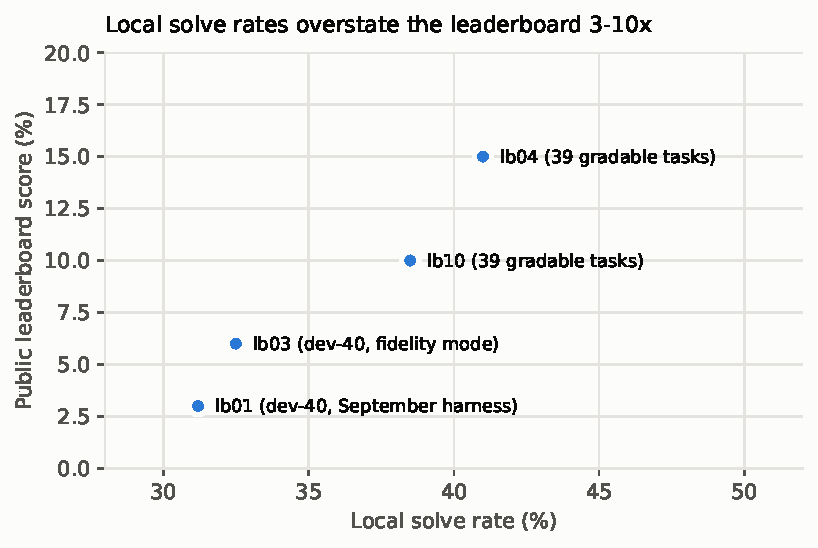
\includegraphics[width=0.66\linewidth]{figures/fig3_local_vs_board.pdf}
\caption{Local solve rate against public leaderboard score for our four scored submissions. The local rate is 3--10$\times$ the board; lb10 and lb04 were within noise locally (15/39 vs 16/39) and 0.05 apart on the board.}
\label{fig:board}
\end{figure}

A screen built from many repositories (we have 142 ingested SWE-rebench tasks) is the obvious next proxy; we did not have time to validate it against the board.

\FloatBarrier
\section{Related work}
SWE-bench~\citep{jimenez2024swebench} defines the task format; agent scaffolds such as SWE-agent~\citep{yang2024sweagent} and the procedural Agentless pipeline~\citep{xia2024agentless} show how much the interface and workflow matter for a fixed model, which our accounting result confirms at the level of a single configuration value. SWE-Gym~\citep{pan2025swegym} trains open models on agent trajectories and reports that self-improvement without a stronger teacher is limited; our LoRA result is a budget-constrained instance. Rejection-sampling fine-tuning follows STaR~\citep{zelikman2022star}; low-rank adaptation of quantized models follows LoRA and QLoRA~\citep{hu2022lora,dettmers2023qlora}. Repetition loops at low temperature are the degeneration described by \citet{holtzman2020degeneration}. Our context-as-cache framing borrows from replacement policies~\citep{belady1966}; serving behaviour depends on vLLM's scheduler and KV management~\citep{kwon2023vllm}. Statistical practice follows~\citet{agarwal2021rliable}.

\section{Limitations and reproducibility}
\label{sec:limits}
The hidden tasks are private, so every local number is a proxy, and our screen over-represents one repository. Most comparisons use one seed on 39--80 tasks; we report intervals and treat $\pm$3 tasks as noise. The L4 time scaling models decode speed only. Board scores are single noisy draws. The temperature-1.0 arm was run only on the 12 tasks lb04 timed out on, and the self-generated LoRA screen was stopped at 32 of 39 tasks; neither has a full paired run. The weight-edit study used the 12B model, not the 31B one.

Everything is reproducible from the repository at \url{https://github.com/shashanka300/runtime-bound}, which contains run manifests and telemetry summaries for every run, the fidelity tooling (scorer-engine environment pinned from the wheelhouse, official harness runner with per-pool wheel caches, compile checker), the gradability sweep, the replay proxy, the timeout and loop analysis, the figure script, and the design-change log (\nolinkurl{docs/design_changes.md}), which records every deviation from the pre-registered plan with the evidence available at the time. No competition data is redistributed.

\bibliographystyle{plainnat}
\bibliography{refs}
\end{document}
